\documentclass[12pt, letterpaper]{article}
\usepackage[ngerman]{babel}
\usepackage{graphicx}
\usepackage{wrapfig}
\usepackage{titlesec}
\usepackage{geometry}
\usepackage[font=scriptsize]{caption}
\usepackage{blindtext}
\usepackage{hyperref}
\usepackage{tabularx}
\usepackage{subcaption}
\usepackage{verbatim}
\usepackage{fancyvrb}
\usepackage{listings}
\usepackage{xcolor}
\usepackage{multirow}
\usepackage{array} % Für die Spaltenbreitenanpassung
\usepackage{booktabs} % Für schönere Tabellen
\usepackage{geometry}
\usepackage{arydshln}
\usepackage{colortbl}

\renewcommand{\lstlistlistingname}{Programmcode}

\geometry{a4paper, margin=2cm}
\hypersetup{
  colorlinks = true,
  linkcolor = black,
  urlcolor = blue,
}

% \captionsetup{justification=raggedright,singlelinecheck=false}
\geometry{
 a4paper,
 total={170mm,257mm},
 left=20mm,
 top=20mm,
 }
%  \titleformat{\section}[display]
%    {\normalfont\bfseries}{}{0pt}{\huge}

\lstdefinestyle{py}{
    language=Python,
    backgroundcolor=\color{white},
    keywordstyle=\color{blue}\bfseries,        % Default Python keywords
    commentstyle=\color{gray}\itshape,         % Comments
    stringstyle=\color{brown},                 % Strings
    %numberstyle=\tiny\color{gray},             % Line numbers
    basicstyle=\ttfamily\small,                % Base font
    identifierstyle=\color{black},             % Default for variable names
    keywordstyle=[2]\color{cyan},              % Functions
    keywordstyle=[3]\color{purple},            % Types
    breaklines=true,
    showstringspaces=false,
    tabsize=4,
    captionpos=b,
    %numbers=left,
    %numbersep=10pt,
    frame=single
}

% Define specific keywords
\lstset{
    morekeywords={import, from, def, return},  % Default Python keywords
    morekeywords=[2]{print, println, len, range, input}, % Functions
    morekeywords=[3]{int, float, str, list, dict, bool} % Types
}


\lstdefinestyle{cpp}{
    language=C,
    backgroundcolor=\color{white},
    keywordstyle=\color{blue}\bfseries,        % Standard Keywords
    commentstyle=\color{green}\itshape,        % Kommentare
    stringstyle=\color{orange},                % Strings
    numberstyle=\tiny\color{gray},             % Zeilennummern
    basicstyle=\ttfamily\small,                % Basis-Schriftart
    identifierstyle=\color{black},             % Standard für Variablennamen
    keywordstyle=[2]\color{cyan},              % Funktionen
    keywordstyle=[3]\color{purple},            % Typen
    breaklines=true,
    showstringspaces=false,
    tabsize=4,
    captionpos=b,
    %numbers=left,
    %numbersep=10pt,
    frame=single
}

% Spezifische Keywords definieren
\lstset{
    morekeywords={if, else, while, return},         % Standard C-Keywords
    morekeywords=[2]{printf, scanf, main, malloc},  % Funktionen (inkl. malloc)
    morekeywords=[3]{int, float, char, double}      % Typen
}

%\lstset{style=pycharm-light}

  
\usepackage{lipsum}  
\graphicspath{ {./Bilder/} }
\author{Oleksii Baida}
\date{Mai 2024}
\begin{document}
\begin{titlepage}
  
\includegraphics[width = 0.25\pdfpagewidth]{./Bilder/FHDO.jpg}
  \begin{center}
    
    \huge \textbf{\textsf{PA2}} \\
    \vspace{3cm}
    \large \textbf{Oleksii Baida}\\
    \textbf{Matrikelnummer 7210384}\\
    \vspace{3cm}
    \large \textbf{Projektarbeit 2}\\
    \vspace{1cm}
    \large \textbf{Bericht}\\
    \vspace{1cm}
    \today
  \end{center}
\end{titlepage}

\tableofcontents
\pagebreak

\section{Einleitung}
\subsection{Gesamtüberblick über das System}
% \par Im Rahmen der Projektarbeit 2 entwickle ich mein System aus der Projektarbeit 1 weiter. Ziel des Projektes ist es, das System aus PA 1 dem Endbenutzer möglichst nahtlos zur Verfügung zu stellen. Die Kernidee des Projekts basiert auf der Entwicklung eines Prototyps, um einen realen Bedarf zu decken.
% \par In der PA 1 habe ich ein Sicherheitssystem für das Haus entwickelt. Das System reagiert auf gefährliche Ereignisse wie Feuer, Gas oder Fremdbewegungen und bietet einen sicheren Zugang zum Haus. Das System ist nur offline verfügbar und hat keine Möglichkeit, den Endbenutzer über die Entfernung zu informieren. In diesem Projekt wird das System durch den Einsatz verschiedener Technologien und Hardwarekomponenten für den Endnutzer über das Internet verfügbar gemacht.
\par Im Rahmen der Projektarbeit 2 entwickele ich ein Sicherheitssystem für das Haus. Das System reagiert auf gefährliche Ereignisse wie Feuer, Gas oder Fremdbewegungen und bietet einen sicheren Zugang zum Haus. Das System ist durch den Einsatz verschiedener Technologien und Hardwarekomponenten für den Endnutzer über das Internet verfügbar. Mein Ziel war es, das System so kabellos und tragbar wie möglich zu machen.
\par Die im Projekt verwendeten Sensoren werden an den Arduino angeschlossen. Den Anschluss der Sensoren habe ich bereits in meiner Projektarbeit 1 \cite{pa1} beschrieben. In diesem Teil des Projektes stelle ich das System dem Endbenutzer über das Internet zur Verfügung. 
\par Die Abbildung \ref{abb:gesamtplan} zeigt den Gesamtaufbau des Systems. Der Arduino ist über eine serielle UART-Schnittstelle mit dem ESP8266 verbunden. Der ESP8266 wird als WLAN-Modul zur MQTT-Kommunikation zwischen dem Arduino und dem Raspberry Pi verwendet. Der Raspberry Pi ist der zentrale Server des Systems. Er stellt einen WLAN-Access-Point zur Verfügung, verwaltet die MQTT-Nachrichten und steuert den Internetzugang. Die Interaktion mit den Endnutzern erfolgt über den Messenger "Telegram". Der Endnutzer wird über die Gefahr in seiner Wohnung informiert und kann bestimmte Systemeinstellungen ändern. 
\par In der vorliegenden Ausarbeitung werden zunächst die verwendeten Hardwarekomponenten, Kommunikationstechnologien sowie Softwareprodukte beschrieben. Im Anschluss erfolgt eine detaillierte Darstellung des Systemaufbaus.
\begin{figure}[h]
  \centering
  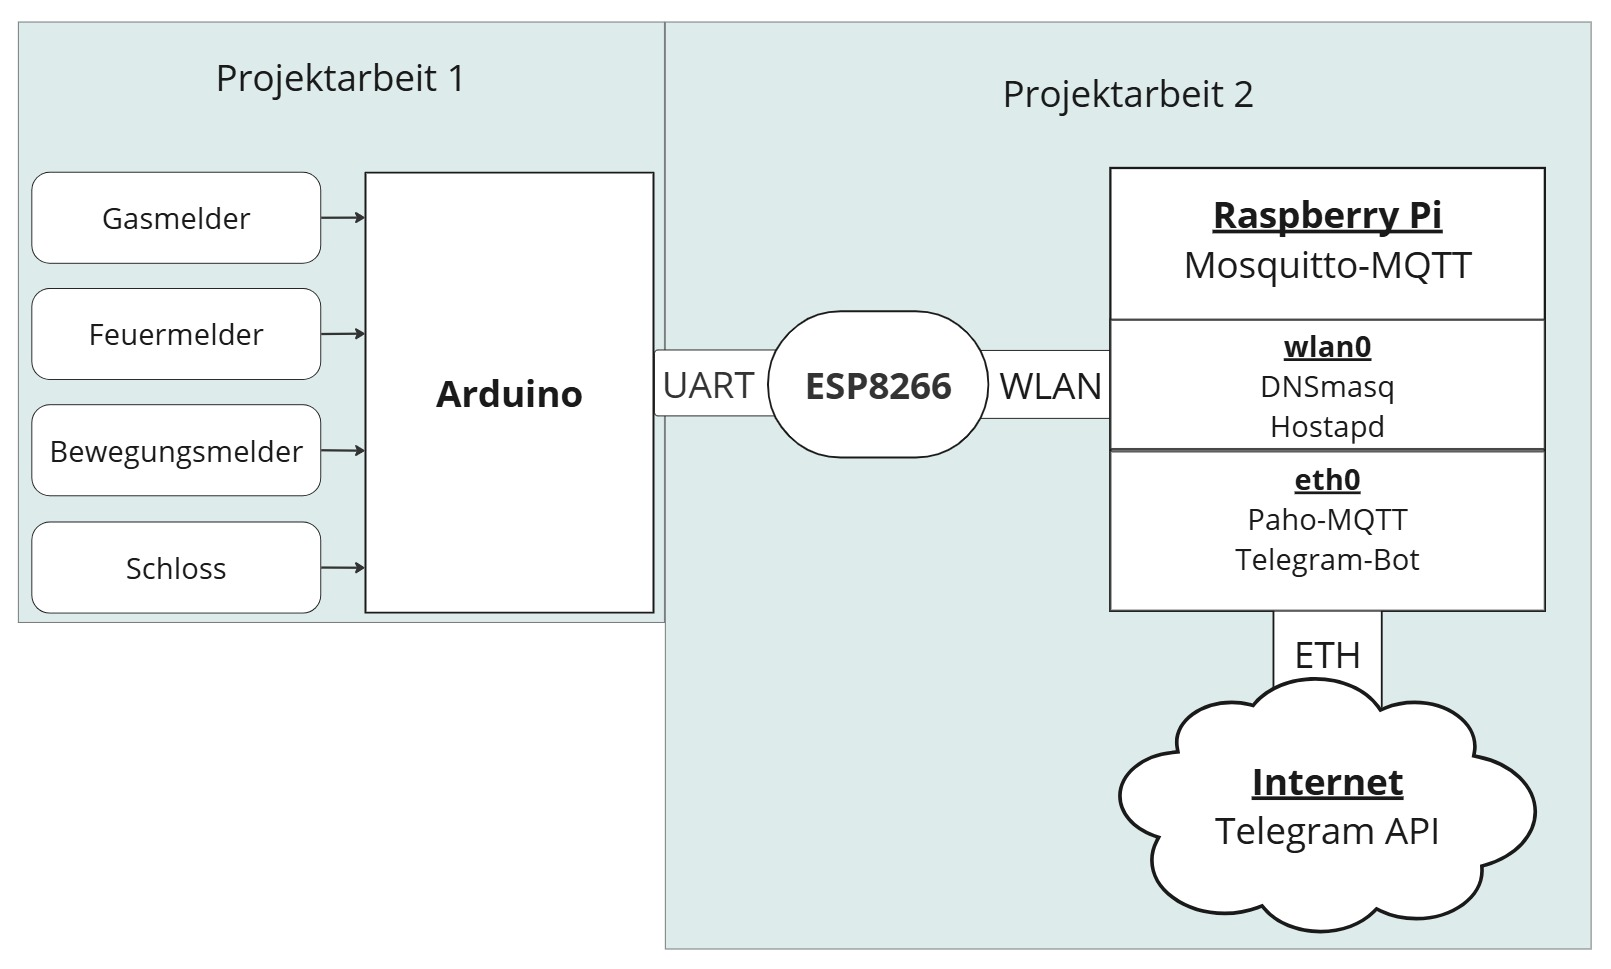
\includegraphics[width=\textwidth]{gesamtplan.jpg}
  \caption{Struktur des Systems}
  \label{abb:gesamtplan}
\end{figure}
\subsection{Verwendete Hardware}
\subsubsection{Raspberry Pi}
\par Im Kern des Systems liegt der Raspberry Pi. Der Raspberry Pi dient als zentraler Server des Systems. Er hat verschiedene Funktionen im System. Der Raspberry Pi dient als MQTT-Broker, um die MQTT-Nachrichten zu verarbeiten. Er stellt einen WLAN-Zugriffspunkt zur Verfügung. Der Raspberry Pi dient auch als Host für den Telegram-Bot. 
\par Für das Projekt verwende ich den Raspberry Pi 1.0 Modell B+. Raspberry Pi ist ein kompakter und kostengünstiger Einplatinencomputer. Die technischen Daten sind in der Tabelle \ref{tbl:raspberry_tech} aufgeführt.
\begin{table}[h!]
  \centering
  \renewcommand{\arraystretch}{1.5}
  \begin{tabular}{|>{\centering\arraybackslash}p{0.5\textwidth}|>{\centering\arraybackslash}p{0.5\textwidth}|}  %{|l|l|}
  \hline
  Modell                               & Raspberry Pi 1.0 Modell B+               \\ \hline
  Prozessor                            & ARM-Prozessor                            \\ \hline
  Arbeitsspeicher (RAM)                & 512 MB                                   \\ \hline
  USB-Ports                            & 4                                 \\ \hline
  MicroSD-Kartensteckplatz             & 1                                 \\ \hline
  HDMI-Anschluss                       & 1                                 \\ \hline
  Ethernet-Anschluss                   & 1                                 \\ \hline
  GPIO-Pins                            & 40                                 \\ \hline
  Wi-Fi                                & Vorhanden                                \\ \hline
  Bluetooth                            & Vorhanden                                \\ \hline
  Stromversorgung                      & 5V Micro-USB-Anschluss                      \\ \hline
  Betriebssystem                       & Raspberry Pi OS \\ &Debian 11 ''Bullseye''             \\ \hline
  \end{tabular}
  \caption{Technische Daten des Raspberry Pi}
  \label{tbl:raspberry_tech}
  \end{table}
\subsubsection{ESP8266}
\par Das System, das ich in PA 1 entwickelt habe, basiert auf Arduino und verfügt über keine Schnittstelle zum Internet. In diesem Projekt verwende ich dafür ein ESP8266 Modul. Der Arduino ist über eine UART-Schnittstelle mit dem ESP8266 verbunden. Das ESP8266 verbindet sich mit dem vom Raspberry Pi bereitgestellten WLAN sowie mit dem MQTT-Broker, der auf dem Raspberry Pi läuft. Dadurch wird eine Verbindung vom Arduino zum Internet über den Raspberry Pi hergestellt.
\par Das ESP8266 ist ein kleines, günstiges WLAN-Modul. Es wurde von Espressif Systems entwickelt. Das Modul ermöglicht die kabellose Verbindung von Mikrocontrollern mit dem Internet. In meinem Projekt verwende ich das ESP8266, um den Arduino drahtlos mit dem Raspberry PI zu verbinden.
\par Das ESP8266 basiert auf einem 32-Bit-Prozessor und hat einen Systemtakt von 80 MHz bis 160 MHz. Das Modul verfügt über 64 kB RAM als Befehlsspeicher und 96 kB RAM als Datenspeicher. Das ESP8266 besitzt keinen internen Flash-Speicher für die Firware. Ansonsten wird die Firmware in einem externen Flash-Speicher abgelegt und wird blockweise in den RAM-Speicher geladen. Je nach Modell verfügt das ESP8266 über verschiedene Schnittstellen wie I/O-Ports und I2C. Ich verwende das Modell mit WLAN und UART. Über den UART-Port wird der Programmcode in das ESP8266 geladen. Das Modul muss mit einer Spannung von 5 V versorgt werden.
\par Das ESP8266 ist mit vielen Programmiersprachen kompatibel. Für die Programmierung des Moduls verwende ich Visual Studio Code mit der PlatformIO Erweiterung. 

\subsection{Verbindungstheorie}
\subsubsection{MQTT}
\par Das MQTT-Protokoll\footnote[1]{Message Queuing Telemetry Transport} ist ein einfaches, effizientes und leichtgewichtiges Nachrichtenprotokoll, das speziell für den Einsatz in IoT-Systemen entwickelt wurde. Es ermöglicht die Kommunikation von Geräten mit geringer Bandbreite und begrenzten Ressourcen. Das Protokoll basiert auf dem Publish-Subscribe-Modell und erfordert daher eine zentrale Instanz, den Broker. Dies ermöglicht es den Geräten, Nachrichten an einen zentralen MQTT-Broker zu senden und von diesem zu empfangen. Die Nachrichten werden unter Topics veröffentlicht, welche Kanäle darstellen, zu denen sich Subscriber registrieren können. Das Backend für das MQTT-Protokoll kann mit NodeRed realisiert werden. NodeRed bietet ein sehr benutzerfreundliches Interface, um die Nachrichten vom Publisher zu empfangen, zu verarbeiten und an ein Endgerät zu senden, wie zum Beispiel einen Telegram-Bot oder ein Cloud-System.
\par MQTT wird aufgrund seiner Unkompliziertheit oft in Smart-Home-Anwendungen verwendet. Es zeichnet sich durch eine gute Zuverlässigkeit aus, da die Nachrichten immer in einer bestimmten Reihenfolge vermittelt werden. Jede Nachricht wird genau einmal gesendet. Obwohl es keine Garantie für die Zustellung der Nachricht gibt, werden Duplikate vermieden. MQTT ermöglicht das Speichern der letzten Nachricht im Topic, wodurch neue Abonnenten diese Nachricht sofort nach der Registrierung zum Topic erhalten. Aus eigener Erfahrung kann ich bestätigen, dass es bei häufigem Senden der Nachrichten keine Probleme mit der Zustellung gibt. Wenn Nachrichten für eine bestimmte Zeit ausbleiben, sollte überprüft werden, ob die Verbindung unterbrochen ist. MQTT bietet Last-Will-und-Testament-Funktion, was ermöglicht dem Broker eine bestimmte Nachricht bei dem Ausfall der Verbindung zu senden. Diese Nachricht kann bei der Registrierung des Subscribers zum Topic definiert werden und wird im Brocker gespeichert, bis er einen Verbindungsausfall erkennt.
\par Bei der Wahl des Protokolls sollten die Entwickler die folgenden Schlüsselpunkte berücksichtigen:
\begin{itemize}
  \item[\textbullet] \textbf{Data latency} –- Wie schnell sollen die Daten übergeben werden? Wie kann man ein Packet vom Startpunkt zum Endpunkt vernünftig übergeben?
  \item[\textbullet] \textbf{Reliability} –- Welche Folgen hat Datenverlust im IoT-System? Wie kann das System zuverlässiger werden?
  \item[\textbullet] \textbf{Bandwidth} –- Wie groß sind Datenmengen, die transportiert werden sollen?
  \item[\textbullet] \textbf{Transport} –- Welches Protokoll ist für den Transport am besten geeignet? Am meisten wird zwischen TCP, UDP und HTTP entschieden.
\end{itemize}

\subsubsection{UART}
\par UART\footnote[2]{Universal Asynchronous Receiver Transmitter} ist eine Hardwarekomponente, die die serielle Datenübertragung bei der Kommunikation zwischen Mikrocontrollern und anderen Geräten ermöglicht. Eine UART-Schnittstelle ist der Standard für serielle Schnittstellen an PCs und Mikrocontrollern und wird zum Senden und Empfangen von Daten über eine Datenleitung verwendet.
\par UART arbeitet asynchron, d.h. es gibt keine gemeinsame Taktverbindung zwischen den kommunizierenden Geräten. Stattdessen wird die Datenübertragung durch Start- und Stoppbits synchronisiert. Diese ermöglichen es dem Empfänger, den Beginn und das Ende eines Datenpakets zu erkennen. Ein typisches Datenpaket besteht aus einem Startbit, gefolgt von einer festgelegten Anzahl von Datenbits (normalerweise 8), einem optionalen Paritätsbit zur Fehlerkontrolle und einem oder mehreren Stoppbits. Der Vorteil besteht darin, dass keine permanente Synchronisation zwischen Empfänger und Sender erforderlich ist. Sie müssen nur für die Dauer der Übertragung synchronisiert sein. Wenn keine Daten zu übertragen sind, setzt der Sender die Leitung auf die Polarität des Stopbits.
\par Ein entscheidender Vorteil der seriellen Kommunikation ist ihre Einfachheit, sowohl in der Implementierung als auch in der Verkabelung. Um die Kommunikation zwischen den Geräten herzustellen, muss die Rx-Leitung (eng. Receiver, Empfänger) eines Gerätes mit der Tx-Leitung (eng. Transceiver, Sender) eines anderen Gerätes verbunden werden. Dadurch entsteht eine Master-Slave-Beziehung zwischen den beiden Geräten, auch wenn sie gleichberechtigt kommunizieren können. Zudem ist UART in den meisten Mikrocontrollern integriert, was die Anwendung vereinfacht und die Kosten minimiert.
\par In meinem Projekt verwende ich eine UART-Schnittstelle für die Verbindung von Arduino und ESP8266.
\subsection{Verwendete Software} 
\subsubsection{Python}
\par Python ist eine weit verbreitete höhere Programmiersprache. Sie wurde 1991 von Guido van Rossum veröffentlicht.
\par Python hat eine klare und leicht lesbare Syntax. Die Strukturierung von Blöcken erfolgt nicht durch geschweifte Klammern, sondern durch Einrückungen. Python unterstützt verschiedene Programmierparadigmen wie objektorientierte, aspektorientierte und funktionale Programmierung. Zudem bietet Python eine dynamische Typisierung.
\par Python ist plattformunabhängig. Der Code von Python-Skripten wird nicht direkt in Maschinencode kompiliert, sondern zur Laufzeit in den Bytecode übersetzt. Der Bytecode ist nicht systemspezifisch, sondern stellt eine Zwischenschicht dar. Der Bytecode wird dann von der Python Virtual Machine (PVM) interpretiert und ausgeführt. Die PVM übernimmt die betriebssystemspezifischen Aufgaben wie Speicherverwaltung, Zugriff auf Prozessoren oder die Nutzung von Systembibliotheken. Dadurch können Python-Programme auf verschiedenen Plattformen ausgeführt werden, sofern eine geeignete PVM für die Plattform vorhanden ist.
\par Die Standardbibliothek von Python umfasst eine umfangreiche Sammlung von Modulen und Funktionen, die auf allen unterstützten Plattformen lauffähig sind. Darüber hinaus steht eine Vielzahl von Drittanbieter-Bibliotheken zur Verfügung, die ebenfalls plattformunabhängig sind. 
\par Im Rahmen meines Projektes werden Python-Skripte für die Behandlung der MQTT-Nachrichten sowie für die Steuerung des Telegram-Bots verwendet. Die Ausführung des Codes erfolgt auf dem Raspberry Pi.
\subsubsection{paho-mqtt}
\par Für die Behandlung der MQTT-Nachrichten, die an den Broker gesendet wurden, wird eine Paho-MQTT-Bibliothek für Python verwendet. Die Bibliothek wurde von der Eclipse Foundation entwickelt und ermöglicht eine einfache und schnelle Kommunikation im MQTT-Protokoll. Sie ist sehr gut für IoT-Anwendungen geeignet. 
\par Durch die Verwendung von Paho-Mqtt können die Nachrichten an bestimmte Topic gesendet werden und der Client kann ein oder mehrere Topics abonnieren. Die Bibliothek bietet eine ereignisorientierte Programmierung, die auf spezifische Ereignisse wie Verbindungsaufbau oder Nachrichteneingang reagiert. Dank der Thread-Sicherheit eignet sich Paho-MQTT gut für Anwendungen, die in einer multithreaded Umgebung arbeiten.
\par Beim Start des Programms muss in der run()-Methode eine loop()-Funktion gestart werden. Sie sorgt dafür, dass Nachrichten empfangen, gesendet und Callback-Funktionen ausgeführt werden, wenn Nachrichten eintreffen oder Verbindungsereignisse auftreten.
\subsubsection{Telegram}
\par Telegram ist ein Cloud-basierter Instant-Messaging-Dienst. Er wurde 2013 von den Brüdern Durov entwickelt. Der Messenger zeichnet sich durch hohe Sicherheit, Flexibilität und Plattformunabhängigkeit aus. Telegram kann auf unterschiedlichen Geräten genutzt werden. Die Chats sowie die Nutzerdaten werden in einer Cloud gespeichert und in Echtzeit synchronisiert. Telegram unterstützt Einzel- und Gruppenchats, Sprach- und Videoanrufe, die Übertragung von Bildern, Videos oder anderen Dateien. Durch den Einsatz einer Ende-zu-Ende-Verschlüsselung in sogenannten "Secret Chats" gewährleistet Telegram eine hohe Datensicherheit. Die regulären Chats werden in der Cloud gespeichert und verschlüsselt übertragen.
\par Was Telegram besonders auszeichnet und bei Entwicklern beliebt macht, ist die Unterstützung von Bots. Bots sind automatisierte Programme, die über Telegram mit Nutzern interagieren können. Bots können zur Automatisierung von Aufgaben, zur Bereitstellung von Informationen oder zur Unterhaltung eingesetzt werden. Die offene API von Telegram ermöglicht es Entwicklern, ihre eigenen Bots zu erstellen und deren Funktionalität an spezifische Anforderungen anzupassen. Die neueste Version unterstützt auch die Nutzung von Webanwendungen direkt über den Bot.
\par Jeder Telegram-Nutzer kann einen Telegram-Bot erstellen. Die Bots werden vom Bot @BotFather verwaltet. Der Benutzer muss @BotFather aufrufen und dann einen neuen Bot erstellen. Dabei wird nach dem Namen und dem Benutzernamen gefragt, der mit “bot” enden muss. Anschließend wird ein Bot erstellt und diesem ein API-Token zugewiesen. Dieses Token wird im Programmcode verwendet, um den Zugriff auf den Bot zu ermöglichen.
\subsubsection{Python-Telegram-Bot}
\label{sec:telegram-bot}
\par Für die Programmierung des Telegram-Bots wird eine \texttt{python-telegram-bot}-Bibliothek verwendet. Die Bibliothek bietet eine umfangreiche API zur Verwaltung der Bot-Funktionalität. Um den Bot zu starten, muss eine Applikation mit dem Token erstellt und auf Polling gesetzt werden.
\par Die Bibliothek unterstützt den Empfang und Versand von Nachrichten in verschiedenen Formaten. Entwickler können den Bot so konfigurieren, dass er auf bestimmte Nachrichten oder Befehle reagiert, indem sie "Handler" definieren, die das Verhalten des Bots steuern. Der Bot kann auch Nachrichten senden, ohne dass der Benutzer im Chat aktiv ist.
\par Ein zentrales Konzept der Bibliothek ist der CommandHandler. Mit Hilfe des CommandHandlers können Bots auf bestimmte Eingaben wie \texttt{/start}, \texttt{/help} oder benutzerdefinierte Befehle reagieren. Dies bietet eine einfache Möglichkeit, die Interaktionen des Bots zu steuern und verschiedene Funktionen zu implementieren. Der Befehl \texttt{/start} wird immer beim ersten Start des Bots vom neuen Benutzer aufgerufen.
\par Die Nachrichten, die der Bot empfängt oder versendet, werden asynchron bearbeitet. Das heißt, jede Funktion, die Nachrichten absendet oder auf die Nachrichten reagirt muss mit \texttt{async}-Befehl deklariert sein. Der Versand der Nachricht muss dann mit \texttt{await}-Befehl erwartet sein. An sonsten bekommt man ein Fehler \"The Funktion was never awaited\".
\par Die Bibliothek unterstützt Webhooks, die eine Kommunikation in Echtzeit ermöglichen. Webhooks ermöglichen es dem Bot, Nachrichten von Telegram direkt über HTTP-Requests zu empfangen, ohne den Server regelmäßig nach neuen Nachrichten abfragen zu müssen.
\par Außerdem bietet die Bibliothek eine Vielzahl von Interaktionen mit dem Benutzer. Es ist möglich eine Inline- oder Antworttastatur zu erstellen, sodass Nutzer vorgefertigte Antworten auswählen können. Die Benutzerverwaltung ist auch in der Bibliothek vorhanden. Entwickler können Benutzerinformationen abrufen, speichern und auf diese Weise personalisierte Erfahrungen bieten.
\par Nach dem Aufbau der Applikation, muss die Polling-Funktion des Bots aufgerufen werden. Polling ist eine Methode, bei der der Bot kontinuierlich die Telegram-Server nach neuen Nachrichten abfragt. Der Bot sendet in regelmäßigen Abständen Anfragen an den Server, um zu prüfen, ob neue Nachrichten eingegangen sind. Dies ist ein einfacher Mechanismus, um den Bot zu betreiben, ohne auf Webhooks angewiesen zu sein.

\section{Raspberry Pi} \label{sec:raspberry}
\par In meinem Projekt verwende ich den Raspberry Pi als zentralen Server des Systems sowie den MQTT-Broker. Die Verbindung zwischen dem ESP8266 und dem Raspberry Pi erfolgt über WLAN. Dazu müssen beide Geräte an ein Netzwerk angeschlossen werden. Hierfür gibt es zwei Möglichkeiten: entweder werden die beiden Geräte über ein Heimnetzwerk mit dem Router verbunden, oder das Netzwerk wird vom Raspberry Pi zur Verfügung gestellt. Für mein Projekt habe ich mich für die zweite Variante entschieden. Der Raspberry Pi wird als ein Access Point konfiguriert und über Ethernet mit dem Internet verbunden. Das ESP8266 verbindet sich dann mit dem MQTT-Broker, der auf dem Raspberry Pi gehostet wird. Der Raspberry übernimmt somit die Rolle eines Routers. Dies hat folgende Vorteile:
\begin{itemize}
  \item Das lokale WLAN-Netzwerk kann direkt am Raspberry Pi konfiguriert werden. Das vereinfacht die Verbindung der angeschlossenen Geräten sowie die Überwachung der Datenübertragung.
  \item Die Sicherheit der Verbindung wird dadurch erhöht, dass das lokale WLAN von außen (aus dem Internet) nicht sichtbar ist. Zusätzlich kann auf dem Raspberry Pi eine Firewall für die Internetverbindung eingerichtet werden.
  \item Das gesamte System ist portabler. Wenn das System an einem anderen Ort installiert wird, muss nur die Internetverbindung mit dem Raspberry Pi eingerichtet werden. Das lokale WLAN muss nicht angepasst werden.
\end{itemize}
\par Weiter unten wird die Einstellung des Raspberry Pi beschrieben.

\subsection{Einrichtung als Access Point}
\par Für die Einrichtung des Raspberry Pi als WLAN Access Point wird das Softwarepaket \texttt{hostapd}\footnote[3]{Host Access Point Daemon} verwendet. Mit Hilfe von hostapd können normale Netzwerkkarten in Access Points umgewandelt werden. Für meine Zwecke muss das Interface \texttt{wlan0} als Access Point umgewandelt werden.
\par Zunächst muss das Paket auf dem Raspberry Pi installiert werden.
\begin{Verbatim}[frame=single]
  sudo apt-get install hostapd
\end{Verbatim}
Für die Konfiguration des Access Points muss die Konfigurationsdatei  erstellt werden. 
\begin{Verbatim}[frame=single]
  sudo nano /etc/hostapd/hostapd.conf
_____________________________________________________________________________
  #Konfigurationsdatei für hostapd
  
  interface=wlan0
  driver=nl80211
  country_code=DE
  ssid=RaspEsp
  hw_mode=g
  channel=6
  wmm_enabled=0
  macaddr_acl=0
  auth_algs=1
  ignore_broadcast_ssid=0
  wpa=2
  wpa_passphrase=mqtt1234
  wpa_key_mgmt=WPA-PSK
  wpa_pairwise=TKIP
  rsn_pairwise=CCMP

  #End
\end{Verbatim}
\par In Bezug auf die Vielzahl an verfügbaren Optionen, die sich für die Konfiguration des hostapd anbieten, habe ich für mein Projekt folgende Einstellungen gewählt: 
\begin{itemize}
  \item[\textbullet] \textbf{interface} --- bezeichnet das Interface, das zu Access Point konfiguriert wird.
  \item[\textbullet] \textbf{driver} --- nl80211 ist der standarte, meistverwendete Driver für \texttt{hostapd}.
  \item[\textbullet] \textbf{country\_code} --- bezeichnet das Land, wo das Netzwerk läuft.
  \item[\textbullet] \textbf{ssid} --- der Name des Netzwerks.
  \item[\textbullet] \textbf{hw\_mode}  --- Operation Mode. 'g' steht für Standard IEEE 802.11g.
  \item[\textbullet] \textbf{channel} --- der verwendete Kanal für die WLAN-Verbindung
  \item[\textbullet] \textbf{wmm\_enabled} --- Wireless Multimedia Extension muss für die WLAN-Verbindung aktiviert sein.
  \item[\textbullet] \textbf{macaddr\_acl} --- Authentifizierung auf Basis des MAC-Protokolls. 0 akzeptiert alle MAC-Adressen, die nicht in Ablehnungsliste sind.
  \item[\textbullet] \textbf{auth\_algs} --- Shared-Key-Authentifizierung
  \item[\textbullet] \textbf{ignore\_broadcast\_ssid} --- Standardeinstellung. Ignoriert Anfragen, die kein vollständiges SSID erhalten.
  \item[\textbullet] \textbf{wpa} --- Wi-Fi Protected Access. Art der Sicherheit des Access Points. Für das Projekt wird WPA 2 verwendet.
  \item[\textbullet] \textbf{wpa\_passphrase} --- das Passwort für den Access Points
  \item[\textbullet] \textbf{wpa\_key\_mgmt, wpa\_pairwise, rsn\_pairwise} --- sind für WPA 2 benötigt.
\end{itemize}
\par Anschließend soll das hostapd automatisch beim Hochfahren starten. Dazu ist es erforderlich, die Einstellungen für den Systemstart anzupassen
\begin{Verbatim}[frame=single]
  sudo nano /etc/default/hostapd

  DAEMON\_CONF="/etc/hostapd/hostapd.conf"
\end{Verbatim}
\par Nun ist der \texttt{hostapd} konfiguriert, aber noch nicht gestartet. Die beiden Befehle starten die \texttt{hostapd}:
\begin{Verbatim}[frame=single]
  sudo systemctl unmask hostapd
  sudo systemctl enable hostapd

  sudo reboot #Neustart des Raspberry Pi
\end{Verbatim}
\par Danach wird ein Neustart des Raspberry Pi empfohlen, um die Änderungen anzuwenden. Der Access Point sollte nun mit entsprechendem SSID auf anderen Geräten sichtbar sein, allerdings ist eine Verbindung zu ihm nicht möglich. Um die Verbindung zu ermöglichen, müssen der DNS- sowie der DHCP-Server auf dem Raspberry Pi eingerichtet werden.

\subsection{Einrichtung des DNS- und DHCP-Servers}
\par Der DNS\footnote[4]{Domain Name System}-Server übersetzt Domains in die IP-Adressen. Der DHCP\footnote[5]{Dynamic Host Configuration Protocol}-Server weist die IP-Adressen den verbundenen Geräten zu. Für die reibungslose Verbindung und Kommunikation müssen beide Server auf dem Raspberry PI eingerichtet werden.
\par Für die Konfiguration des DNS-Servers sowie des DHCP-Servers wird das Softwarepaket \texttt{dnsmasq} verwendet. Das Paket ermöglicht eine einfache und schnelle Konfiguration der beiden Server auf Linux-basierten Systemen.
\par In der Konfigurationsdatei sind eine Vielzahl an die Optionen für die Einstellung des DNS-Servers vorgegeben, wobei lediglich ein Teil davon für die Bearbeitung relevant ist.
\begin{Verbatim}[frame=single]
  sudo nano /etc/dnsmasq.conf
_____________________________________________________________________________
  #Konfigurationsdatei für DNS-Server

  interface=wlan0
  bind-dynamic
  domain-needed
  bogus-priv
  dhcp-range=192.168.1.100,192.168.1.110,255.255.255.0,12h

  #End
\end{Verbatim}
\begin{itemize}
  \item[\textbullet] \textbf{interface} --- definiert Interface, an welchem der DNS-Server fungiert.
  \item[\textbullet] \textbf{bind-dynamic} --- erlaubt die Verbindung nur mir exsistierenden Inrefaces.
  \item[\textbullet] \textbf{domain-needed} --- ignoriert DNS-Anfragen ohne Domänennamen. 
  \item[\textbullet] \textbf{bogus-priv} --- die DNS-Anfragen aus lokalem Netzwerk werden nicht an Haupt-DNS-Server weitegeleitet.
  \item[\textbullet] \textbf{dhcp-range} --- gibt den Bereich der IP-Adressen für DHCP-Server an.
\end{itemize}
\par Anschließend muss der DHCP-Server eingerichtet werden.
\begin{Verbatim}[frame=single]
  sudo nano /etc/dhcpcd.conf
_____________________________________________________________________________
  #Konfigurationsdatei für DHCP-Server

  nohook wpa_supplicant
  interface=wlan0
  static ip_address=192.168.1.10/24
  static routers=192.168.1.1

  #End
\end{Verbatim}
\par Entsprechend den oben beschriebenen Einstellungen werden die IP-Adressen von 192.168.1.100 bis 192.168.1.110 durch den DHCP-Server verteilt und laufen nach 12 Stunden automatisch ab. Für den Host (Raspberry Pi) ist die IP-Adresse 192.168.1.10 reserviert. Default-Gateway hat die IP-Adresse 192.168.1.1 
\subsection{MQTT-Broker}
\par Der MQTT Broker ermöglicht die Kommunikation zwischen den MQTT-Geräten. Der Broker empfängt Nachrichten von sogenannten "Publishern" und leitet sie an "Subscriber" weiter. Die Subscriber müssen sich für bestimmte Themen (Topics) registrieren.
\par In meinem System läuft der MQTT-Broker auf dem Raspberry Pi. Für die Einrichtung des Brokers wird das Softwarepaket \texttt{mosquitto}\footnote[6]{https://mosquitto.org/} verwendet. Mosquitto erlaubt schnelle und einfache Einstellung und Verwaltung von MQTT-Broker. 
\par 
\begin{enumerate}
  \item Installation:
\begin{Verbatim}[frame=single]
  sudo apt install mosquitto mosquitto-clients
\end{Verbatim}
\item Autostart einschalten:
\begin{Verbatim}[frame=single]
  sudo systemctl enable mosquitto
  sudo systemctl start mosquitto
\end{Verbatim}
\item Konfiguration:
\begin{Verbatim}[frame=single]
  sudo nano /etc/mosquitto/mosquitto.conf
_________________________________________________________________________
  #Konfigurationsdatei für mosquitto

  pid_file /run/mosquitto/mosquitto.pid

  persistence true
  persistence_location /var/lib/mosquitto/

  log_dest file /var/log/mosquitto/mosquitto.log

  include_dir /etc/mosquitto/conf.d

  listener 1883
  allow_anonymous true
\end{Verbatim}
\par allow\_anonymous für die Ersteinrichtung und zu Testzwecken einschalten. Die Konfiguration der Benutzer erfolgt weiterhin im Text LINK.
\item Konfigurationsdatei speichern \texttt{Strg+O} und schließen \texttt{Strg+X} und Mosquitto neu starten 
\begin{Verbatim}[frame=single]
  sudo systemctl restart mosquitto
\end{Verbatim}
  \item Testen. Ein Subscriber für Topic registrieren: 
\begin{Verbatim}[frame=single]
  mosquitto_sub -h localhost -t <DEIN_TOPIC>
\end{Verbatim}
\par Neues Fenster öffnen \texttt{Strg+T} und über einen Publisher eine Nachricht in das Topic senden.
\begin{Verbatim}[frame=single]
  mosquitto_pub -h localhost -t <DEIN_TOPIC> -m "MEINE 1. MQTT-NACHRICHT"
\end{Verbatim}
\par Nach dem Parameter -t (Topic) keine Klammern setzen. Nach dem Parameter -m (Message) den Text der Nachricht in Klammern setzen.
\subsubsection{MQTT-Flow}
\par In der Tabelle sind die Topic mit Nachrichten gelistet:
\end{enumerate}
\begin{table}[h!]
  \centering
  \renewcommand{\arraystretch}{1.5}
  \begin{tabular}{|>{\centering\arraybackslash}p{2cm}|>{\centering\arraybackslash}p{3cm}|>{\centering\arraybackslash}m{11cm}|}
  \hline
  \textbf{Topic} & \textbf{Nachricht} & \textbf{Definition} \\ \hline
  \multirow{7}{*}{\centering alarm}  & fire\_start   & Feuersensor hat das Feuer erkannt.\\  \cline{2-3}
                          & fire\_go      & Feuersensor erkennt weiter das Feuer.\newline Wird 1 Mal Pro Sekunde ausgegeben.\\ \cline{2-3}
                          & fire\_stop    & Feuersensor erkennt kein Feuer mehr.\newline Das Feuer wurde gelöscht.\\\cline{2-3}
                          & gas\_start    & Gassensor hat erhöhte Konzentration von Gas erkannt\\ \cline{2-3}
                          & gas\_go       & Gassensor erkennt das Gas weiter.\newline Wird 1 Mal pro Sekunde ausgegeben\\     \cline{2-3}
                          & gas\_stop     & Gassensor erkennt kein Gas mehr. Luft ist wieder rein. \\ \cline{2-3}
                          & pir\_move     & Bewegungssensor hat eine Bewegung erkannt\\  \hline 
  \multirow{5}{*}{pin}    & pin\_wrong    & Eine falsche PIN wurde eingegeben\\ \cline{2-3}
                          & pin\_correct  & Die richtige PIN wurde eingegeben \\ \cline{2-3}
                          & pin\_change\_start  & Die PIN-Änderung hat angefangen \\ \cline{2-3}
                          & pin\_change\_stop   & Die PIN-Änderung wurde abgebrochen \\ \cline{2-3}
                          & pin\_change\_suc    & Die PIN wurde erfolgreich geändert \\ \hline
                         
  \end{tabular}
  
  \caption{MQTT-Topics mit möglichen Nachrichten}
  \end{table}
\subsection{Telegram Bot und Paho-Client}
\par Bisher kann der Raspberry Pi einen WLAN-Access-Point zur Verfügung stellen und MQTT-Nachrichten empfangen. Es fehlt noch eine Schnittstelle zum Endbenutzer, die ebenfalls auf dem Raspberry Pi implementiert wird. Ich habe mich für ein Telegram-Bot entschieden. Dazu muss ein Verwaltungsmechanismus für die MQTT-Nachrichten entwickelt werden. Für diese Zwecke verwende iche ein Python-Bibliothek \texttt{"paho-mqtt"}.
\par Die Struktur ist wie folgendes aufgebaut(SPÄTER WEG, GESAMTSTRUKTUR WIRD AM ANFANG BESCHRIEBEN):
\begin{Verbatim}[frame=single]
  |-python-scripts
  |
  |--app.py
  |--mqtt.py
  |--tg-bot.py
\end{Verbatim}

\subsubsection{Paho-MQTT}
\par Die Implementierung des Paho-Clients erfolgt in der Datei \texttt{mqtt.py}. Folgende Bibliotheke(????) müssen importiert werden:
\begin{lstlisting}[frame=single, style=py, caption={mqtt.py: imports}]
  from paho.mqtt import client as mqtt_client
  import threading
  from queue import Queue
\end{lstlisting}
\par Um die Erstellung eines Objekts zu erlauben muss ein Klass MqttBroker deklariert werden. Der Konstruktor ist in der Funktion \texttt{\_\_init\_\_} definiert:
\begin{lstlisting}[frame=single,style=py, caption={mqtt.py: \_\_init\_\_()}]
  def __init__(self, queue, broker, port, topic, client_id):
    threading.Thread.__init__(self)
    self.queue = queue
    self.broker = broker
    self.port = port
    self.topic = topic

    self.client = mqtt_client.Client(client_id)
    self.client.on_connect = self.on_connect
    self.cleint.on_message = self.on_message
    self.client.on_disconnect = self.on_disconnect
    self.client.connect(self.broker, self.port)
\end{lstlisting}
\par Konstruktor-Parameter:
\begin{itemize}
  \item[\textbullet] \textbf{queue} -- ein Queue-Objekt. Queue wird in der Startklasse app.py initialisiert. Erlaubt Threadsafe Synchronisation des MQTT-Broker und Telegram-Bots.
  \item[] \item[\textbullet] \textbf{broker} -- String. IP-Adresse des MQTT-Brokers. In meinem Fall \texttt{localhost} auf dem Raspberry Pi.
  \item[\textbullet] \textbf{port} -- Integer. Port, auf den der MQTT-Broker hört.
  \item[\textbullet] \textbf{topic} -- String-Array. Topics, zu dem sich der MQTT-Broker anmeldet. Kann ein oder mehrere Topic sein.
  \item[\textbullet] \textbf{client\_id} -- String. Name des Clients.
\end{itemize}
\par Sowohl MqttBroker als auch Telegram-Bot verwenden eine Endlosschleife, um kontinuierlich Anfragen an den Server bzw. an den Broker zu senden. Damit die beiden Programme parallel laufen können, müssen sie in getrennten Threads gestartet werden. Die Threads werden direkt bei der Initialisierung des Klassenobjekts gestartet. Danach wird ein \texttt{mqtt\_client}-Objekt mit übergebener Id initialisiert. Anschließend werden die Callback-Funktionen für ausgewählte Ereignisse deklariert und dem Client zugewiesen. Als letztes verbindet sich der Client mit dem Broker.
\par Nach der Initialisierung muss das Programm mit der Funktion \texttt{run()} gestartet werden.
\begin{lstlisting}[frame=single, style=py, caption={mqtt.py: run()}]
  def run(self):
    # mehrere Topic abonnieren
    for t in self.topic:
      self.client.subscribe(t)
    
    self.client.loop_start()
\end{lstlisting}
\par Die \texttt{loop\_start()}-Funkltion startet eine Endlosschleife und fragt den MQTT-Broker stätig an den Nachrichten. Beim Nachrichteneingang wird die Funktion \texttt{on\_message()} aufgerufen. 
\begin{lstlisting}[style=py, caption={mqtt.py: on\_message()}]
  def on_message(self, client, userdata, msg):
    mes = str(msg.payload.decode('utf-8'))
    message = {'topic': msg.topic, 'text': mes}
    self.queue.put(message)
\end{lstlisting}
\par Als Parameter werden die Client- und Benutzerdaten sowie die Nachricht selbst übergeben. Die empfangene Nachricht wird zunächst dekodiert, um den Text in einem lesbaren Format zu erzeugen. Text und Topic der Nachricht werden in einem Dictionary gespeichert und an die Queue übergeben. Der Telegram-Bot kann nun dieses Dictionary problemlos und nahezu in Echtzeit empfangen.
\subsubsection{Telegram-Bot}
\par Für die Implementierung des Telegram-Bots wird eine Python-Bibliothek verwendet. Die Implementierung erfolgt in der Datei \texttt{tg\_bot.py}. In dieser Datei wird die Klasse \texttt{Bot} deklariert, die von der \texttt{threading.Thread} erbt. Zunächst sind folgende Imports erforderlich:
\begin{lstlisting}[style=py,caption={tg\_bot.py: imports}]
  from telegram import Update
  from telegram.ext import filters, ApplicationBuilder, CommandHandler, MessageHandler, CallbackContext
  import threading
  from queue import Queue, Empty

  class Bot(threading.Thread):
  ...
\end{lstlisting}
\par Dem Konstruktor muss ein Queue-Objekt und ein Telegram-Token übergeben werden. Das Token ermöglicht dem Programm den Zugriff auf den Telegram-Bot. In der Klasse \texttt{Bot} werden die Callback-Funktionen für die Reaktion auf empfangene Benutzerbefehle und MQTT-Nachrichten deklariert.
\par Der Bot wird mit dem Aufruf der \texttt{run()}-Funktion gestartet:
\begin{lstlisting}[style=py, caption={tg\_bot.py: run()}]
  def run(self):
    self.application = ApplicationBuilder().token(self.token).build()
    # Haendler fuer die Benutzerbefehle
    self.application.add_handler(
        CommandHandler('start', self.command_start)
    )
    
    job_queue = self.application.job_queue
    if job_queue:
      job_queue.run_repeating(self.wait_mqtt_message, interval = 1)

    self.application.run_polling()
\end{lstlisting}
\par Zunächst muss die Applikation erstellt werden. Danach können die in den entsprechenden Funktionen deklarierten Handler den ausgewählten Ereignissen zugewiesen werden. Anschließend wird eine \texttt{job\_queue} gesucht. Das \texttt{job\_queue} ist ein Queue-Objekt und erlaubt den asynchronen Zugriff auf die Shared Queue. Wenn ein \texttt{job\_queue} gefunden wurde, wird die Queue mit einem Intervall von 1 Sekunde nach neuen Nachrichten abgefragt. Zuletzt muss die Funktion \texttt{run\_polling()} aufgerufen werden.
\begin{lstlisting}[frame=single,style=py,caption={tg\_bot.py: wait\_mqtt\_message()}]
  async def wait_mqtt_message(self, context: CallbackContext):
    try:
      mqtt_message = self.queue.get_nowait()
      await self.handle_mqtt_message(mqtt_message)
      self.queue.task_done()
    except Empty:
      # kein neuer Eingang in Queue
      pass
\end{lstlisting}
\par Die Funktion \texttt{wait\_mqtt\_message} sucht nach neuen Einträgen in der Queue. Die Funktion enthält einen Try-Except-Block. Wenn keine neuen Einträge gefunden werden, läuft das Programm ohne Unterbrechung weiter. Wird ein neuer Eintrag gefunden, so wird dieser in \texttt{mqtt\_message} gespeichert und der Funktion \texttt{handle\_mqtt\_message} übergeben. In dieser Funktion wird die eingehende Nachricht verarbeitet und eine Meldung an den Bot ausgegeben.
\section{ESP8266} \label{sec:esp}

\subsection[Arduino-ESP8266]{Verbindung von ESP8266 und Arduino}
\par Die Verbindung zwischen Arduino und ESP8266 kann auf unterschiedliche Weise hergestellt werden. Im Rahmen meines Projekts erfolgt die Verbindung über eine serielle UART-Schnittstelle.
\par Der Arduino verfügt über RX- und TX-Pins (Pin 0 und 1) für die serielle Kommunikation. Der RX-Pin des Arduino muss mit dem TX-Pin auf dem ESP8266 verbunden werden und der TX-Pin umgekehrt.In der Folge können die Daten des Arduino über die Funktion Serial.print() an das Modul ESP8266 über die serielle Schnittstelle übermittelt werden. Dabei ist zu berücksichtigen, dass bei einer Verbindung des Arduino mit einem Rechner über den USB-Port der Arduino den USB-Port als serielle Schnittstelle definiert. Infolgedessen werden keine Daten über die TX- bzw. RX-Ports übergeben. Daher ist eine Versorgung des Arduino mittels eines Netzteiles mit 5 V erforderlich.
\par Aufgrund der Weiterleitung der Daten vom Arduino über die MQTT-Verbindung ist eine entsprechende Berücksichtigung der jeweiligen Formatierung erforderlich. Der Arduino übermittelt die Befehle durch die serielle Schnittstelle mit dem Format "topic:message". Dies erleichtert dem ESP8266 die Verarbeitung der empfangenen Nachricht sowie deren Weiterleitung mit dem entsprechenden Topic. Weiter unten ist der Programmcode für die Verarbeitung der Daten von Arduino zu sehen. 
\begin{lstlisting}[frame=single, style=cpp,caption={ESP8266: readSerialData()}]
  void readSerialData()
  {
    if (Serial.available() > 0)
    {
      String readString = "";
      // Lese Daten aus Serial als String ab
      readString = Serial.readStringUntil('\n');
      
      if (sizeof(readString) > buss_serial)
      {
        return;
      }
      // String in char-Feld konvertieren
      char readSerialChar[readString.length() + 1];
      readString.toCharArray(readSerialChar, readString.length() + 1);
      // Suche Position von ':'
      char *delim_pos = strchr(readSerialChar, ':');
      if (delim_pos != NULL)
      {
        size_t topic_length = delim_pos - readSerialChar;
        char topic[topic_length + 1];
        strncpy(topic, readSerialChar, topic_length);
        topic[topic_length] = '\0';
        char *message = delim_pos + 1;
        // MQTT-Nachricht senden
        mqttClient.publish(topic, message);
      }
      else // kein : gefunden
      {
        Serial.print("FALSCHES FORMAT");
        return;
      }
    }
  }
\end{lstlisting}
\subsection[ESP8266-Raspberry Pi]{ESP8266 als Schnittstelle für die MQTT-Verbindung}
\par In meinem Projekt verwende ich das ESP8266 für die Erstellung der MQTT-Verbindung zwischen Arduino und Raspberry Pi. Wie oben beschrieben, wird der Raspberry Pi als MQTT-Broker und WLAN-Access-Point eingerichtet. Das ESP8266 muss sich mit dem Zuganspunkt von Raspberry Pi verbinden und eine MQTT-Verbindung zu dem Broker erstellen. Außerdem muss das ESP8266 die Daten von Arduino erhalten.
\subsubsection{Verbindung mit WLAN}
\par Zunächst ist eine Verbindung des ESP8266 mit dem vom Raspberry Pi bereitgestellten WLAN erforderlich. Für diesen Zweck wird die Bibliothek \texttt{ESP8266WIFI.h} verwendet. Es muss ein Objekt \texttt{WifiClient} und zwei konstanten Variablen \texttt{WIFI\_SSID} und \texttt{WIFI\_PASSWORD} erstellt werden. In der Konstante \texttt{WIFI\_SSID} wird der Name des WLAN-Netzwerks gespeichert und in der Konstante \texttt{WIFI\_PASSWORD} wird das Passwort gespeichert.
\par Die Verbindungsroutine ist in der Funktion \texttt{connect\_wifi()}  zu sehen. Diese Funktion wird beim Start des Moduls in der \texttt{setup()}-Funktion aufgerufen.
\begin{lstlisting}[frame=single, style=cpp,caption={ESP8266: connect\_wifi()}]
  void connect_wifi()
{

  delay(10);
  Serial.println();
  Serial.print("Connecting to ");
  Serial.println(WIFI_SSID);

  WiFi.mode(WIFI_STA);
  WiFi.begin(WIFI_SSID, WIFI_PASSWORD);

  while (WiFi.status() != WL_CONNECTED)
  {
    delay(500);
    Serial.print(".");
  }

  Serial.println("");
  Serial.println("WiFi connected");
  Serial.println("IP address: ");
  Serial.println(WiFi.localIP());
}
\end{lstlisting}
\par Das ESP8266 versucht jede 200 Milisekunden sich mit dem WLAN zu verbinden. Die Serial-Ausgaben in der Konsole sind nur für die Testzwecken benötigt. 
\subsubsection{Verbindung mit dem MQTT-Broker}
\par Für die Verbindung des ESP8266 mit dem MQTT-Broker wird eine Bibliothek \texttt{PubSubClient.h} verwendet. Es ist erforderlich, dass der MQTT-Broker mit dem gleichen Netzwerk wie das ESP8266 verbunden ist. In meinem System läuft der Broker auf dem Raspberry Pi und das WLAN wurde auch vom Raspberry Pi zur Verfügung gestellt. So befinden sich die beiden Module in einem Netzwerk. 
\par Im Programmcode am ESP8266 muss ein Objekt \texttt{PubSubClient} erstellt werden. Als Parameter wurde den \texttt{WifiClient} übergeben. In der konstanten Variable \texttt{MQTT\_BROKER\_ADRRESS} ist die IP-Adresse des Brokers und in der Variable \texttt{MQTT\_PORT} ist die Portnummer gespeichert. Die Verbindungsroutine ist in die Funktion \texttt{connect\_mqtt()} eingepackt. Diese Funktion wird beim Start vom ESP8266 in der \texttt{setup()}-Funktion aufgerufen.
\begin{lstlisting}[frame=single, style=cpp, caption={ESP8266: connect\_mqtt()}]
  void connect_mqtt()
  {
    Serial.print("\nConnecting ESP to MQTT Broker with IP: ");
    Serial.print(MQTT_BROKER_ADRRESS);
    while (!mqttClient.connected() & WiFi.status() == WL_CONNECTED)
    {
      if (mqttClient.connect(CLIENT_ID)) mqttClient.subscribe(SUBSCRIBE_TOPIC);
      else delay(1000);
    }
  }
\end{lstlisting}
\par Nach erfolgreicher Erstellung der Verbindung mit dem MQTT-Broker muss das ESP8266 das Topic \texttt{UBSCRIBE\_TOPIC} abonnieren, um die Befehle von dem Broker zu erhalten. Das ermöglicht beideseitige Kommunikation zwischen ESP8266 und MQTT-Broker.
\par Sobald das ESP8266 die Daten von dem Arduino empfängt, wird die MQTT-Nachricht an den MQTT-Broker mit dem Befehl \texttt{mqttClient.publish(topic, message)} versandt.
\par Die Verarbeitung der empfangenen Nachricht erfolgt in der \texttt{callback}-Funktion. Für die Testzwecken wird die erhaltene Nachricht in die Konsole ausgegeben. Für die Zukunft ist geplant, die Netzwerkkonfiguration sowie MQTT-Clients auf dem ESP8266 über MQTT-Nachrichten zu steuern.

\begin{lstlisting}[frame=none, style=cpp, caption={ESP8266: callback()},captionpos=b]
  void callback(char *topic, byte *payload, unsigned int length)
{
  Serial.print("Nacricht erhalten. Topic: ");
  Serial.print(topic);
  Serial.print(" Text: ");
  for (int i = 0; i < length; i++)
  {
    Serial.print((char)payload[i]);
  }
  Serial.println();
}
\end{lstlisting}
\newpage

\section{Quellen}
\begin{thebibliography}{20}
  \bibitem{pa1}
  O. Baida,
  \textit{Anbindung der Sensoren und Aktoren an den Arduino zur Realisierung eines Sicherheitssystems},
  Projektarbeit 1, 2024.

  \bibitem{code}
  O. Baida, Programmcode für PA2: \url{https://github.com/oleksiibaida/PA2.git}
  \par \textbf{Links zur verwendeten Hardware:}
  \bibitem{arduino}
  Arduino.cc, \textit{Arduino UNO}, \url{https://docs.arduino.cc/hardware/uno-rev3/}
  \bibitem{raspi}
  Raspberry Pi Foundation, \textit{Raspberry Pi 1 B+}, \url{https://www.raspberrypi.com/products/raspberry-pi-1-model-b-plus/}
  \bibitem{esp8266}
  Espressif, \textit{ESP8266}, \url{https://www.espressif.com/}
  \par \textbf{Links zur verwendeten Software:}
  \par Linux-Packete:
  \bibitem{hostapd}
  Jouni Malinen, \textit{hostapd}, \url{https://w1.fi/hostapd/}, Zugriff am: 19. September 2024.
  \bibitem{dnsmasq}
  Simon Kelley, \textit{dnsmasq}, \url{https://dnsmasq.org/doc.html}, Zugriff am: 20. September 2024.
  \bibitem{mosquitto}
  Eclipse Foundation, \textit{Eclipse Mosquitto}, \url{https://mosquitto.org/}
  \par \textbf{Links zur ESP- und Arduino-Bibliotheken}
  \bibitem{pubsub} 
  Knolleary, \textit{PubSubClient}, \url{https://pubsubclient.knolleary.net/}, Zugriff am: 21. Oktober 2024.
  \par \textbf{Links zur Python-Bibliotheken}
  \bibitem{paho}
  Pierre Fersing, Roger Light \textit{paho-mqtt}, \url{https://pypi.org/project/paho-mqtt/}, Zugriff am: 21. Oktober 2024.
  \bibitem{tgbot}
  Open Source, \textit{python-telegram-bot}, \url{https://docs.python-telegram-bot.org/en/v21.6/}
  \bibitem{queue}
  Python Software Foundation, \textit{queue}, \url{https://docs.python.org/3/library/queue.html}
\end{thebibliography}



\listoffigures
\addcontentsline{toc}{section}{Abbildungsverzeichnis}

\listoftables
\addcontentsline{toc}{section}{Tabellenverzeichnis}
\lstlistoflistings
\addcontentsline{toc}{section}{Programmcode}
\end{document}